% 1999 上海文科 Q8：按固定扫描页重绘；实线为工序，虚线为零工时虚活动。
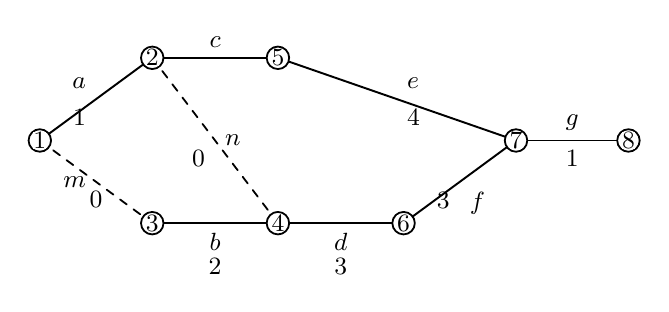
\begin{tikzpicture}[>=stealth, line join=round, line cap=round, scale=0.84,
  every node/.style={font=\small}]
  \tikzset{activity/.style={->, line width=0.7pt}, dummy/.style={->, dashed, line width=0.65pt}}
  \coordinate (n1) at (0,0);
  \coordinate (n2) at (1.7,1.25);
  \coordinate (n3) at (1.7,-1.25);
  \coordinate (n4) at (3.6,-1.25);
  \coordinate (n5) at (3.6,1.25);
  \coordinate (n6) at (5.5,-1.25);
  \coordinate (n7) at (7.2,0);
  \coordinate (n8) at (8.9,0);

  \draw[activity] (n1)--node[above left] {$a$} node[below left] {$1$} (n2);
  \draw[dummy] (n1)--node[left] {$m$} node[below] {$0$} (n3);
  \draw[activity] (n3)--node[below] {$b$} node[below=9pt] {$2$} (n4);
  \draw[dummy] (n2)--node[right] {$n$} node[below left] {$0$} (n4);
  \draw[activity] (n2)--node[above] {$c$} (n5);
  \draw[activity] (n4)--node[below] {$d$} node[below=9pt] {$3$} (n6);
  \draw[activity] (n5)--node[above right] {$e$} node[below right] {$4$} (n7);
  \draw[activity] (n6)--node[below right] {$f$} node[below left] {$3$} (n7);
  \draw[activity] (n7)--node[above] {$g$} node[below] {$1$} (n8);

  \foreach \name in {n1,n2,n3,n4,n5,n6,n7,n8} {
    \draw[fill=white, line width=0.65pt] (\name) circle (0.17);
  }
  \node[fill=white,inner sep=0pt] at (n1) {1};
  \node[fill=white,inner sep=0pt] at (n2) {2};
  \node[fill=white,inner sep=0pt] at (n3) {3};
  \node[fill=white,inner sep=0pt] at (n4) {4};
  \node[fill=white,inner sep=0pt] at (n5) {5};
  \node[fill=white,inner sep=0pt] at (n6) {6};
  \node[fill=white,inner sep=0pt] at (n7) {7};
  \node[fill=white,inner sep=0pt] at (n8) {8};
\end{tikzpicture}
